\addtocontents{toc}{\protect\setcounter{tocdepth}{1}}
\makeatletter
\addtocontents{toc}{%
  \begingroup
  \let\protect\l@chapter\protect\l@section
  \let\protect\l@section\protect\l@subsection
}
\makeatother

\chapter{Native versus cross-platform appearance} \label{a:native_cross}

    \begin{figure}[ht]
        \centering
             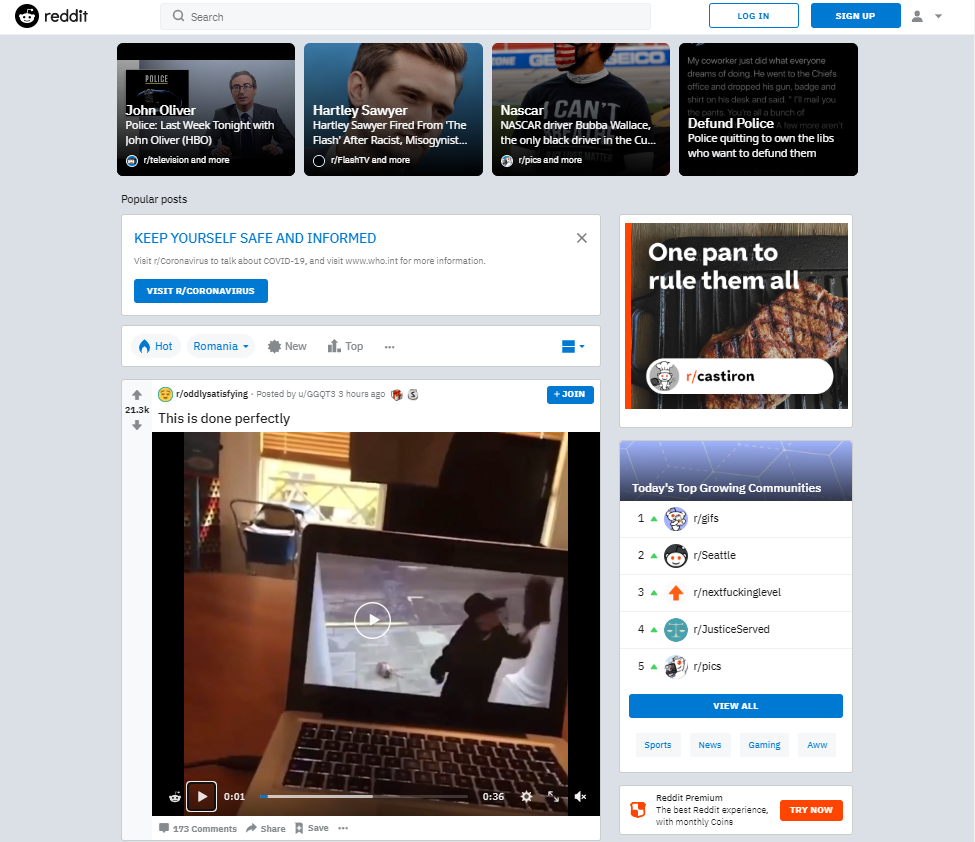
\includegraphics[width=0.95\textwidth]{figures/reddit/reddit_web.png}
        \caption{Official Reddit website}
        \label{a:fig:reddit_web}
    \end{figure}
  
    \begin{figure}[ht]
        \centering
             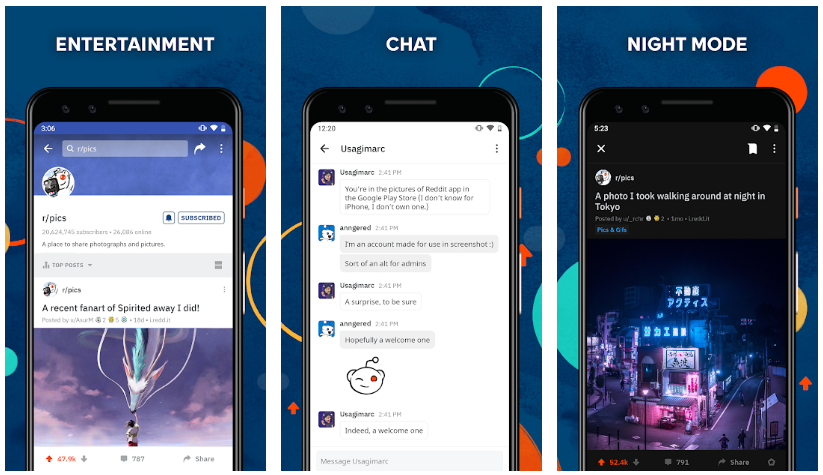
\includegraphics[width=\textwidth]{figures/reddit/reddit_android.png}
        \caption{Official Android Reddit application}
        \label{a:fig:reddit_android}
    \end{figure}
    
    \begin{figure}[ht]
        \centering
             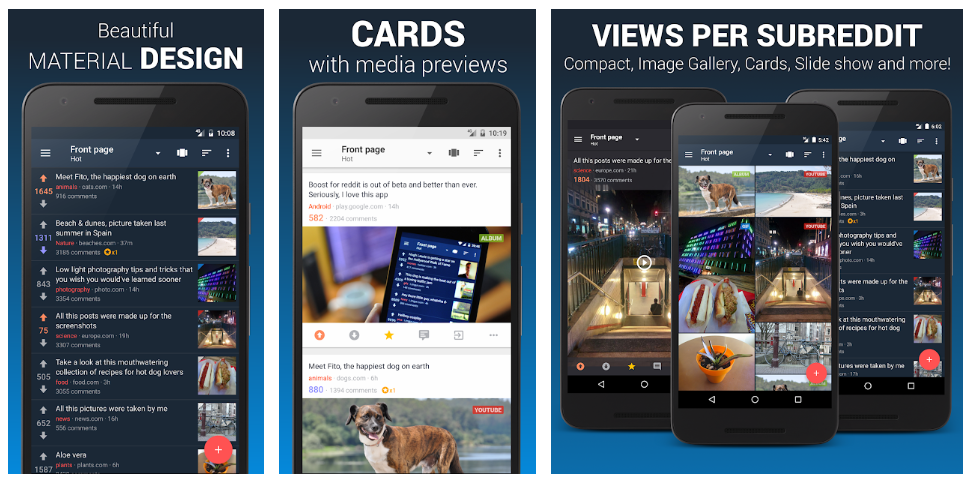
\includegraphics[width=\textwidth]{figures/reddit/reddit_boost.png}
        \caption{Boost for Reddit, an unofficial Android application}
        \label{a:fig:reddit_boost}
    \end{figure}
    
    \begin{figure}[ht]
        \centering
             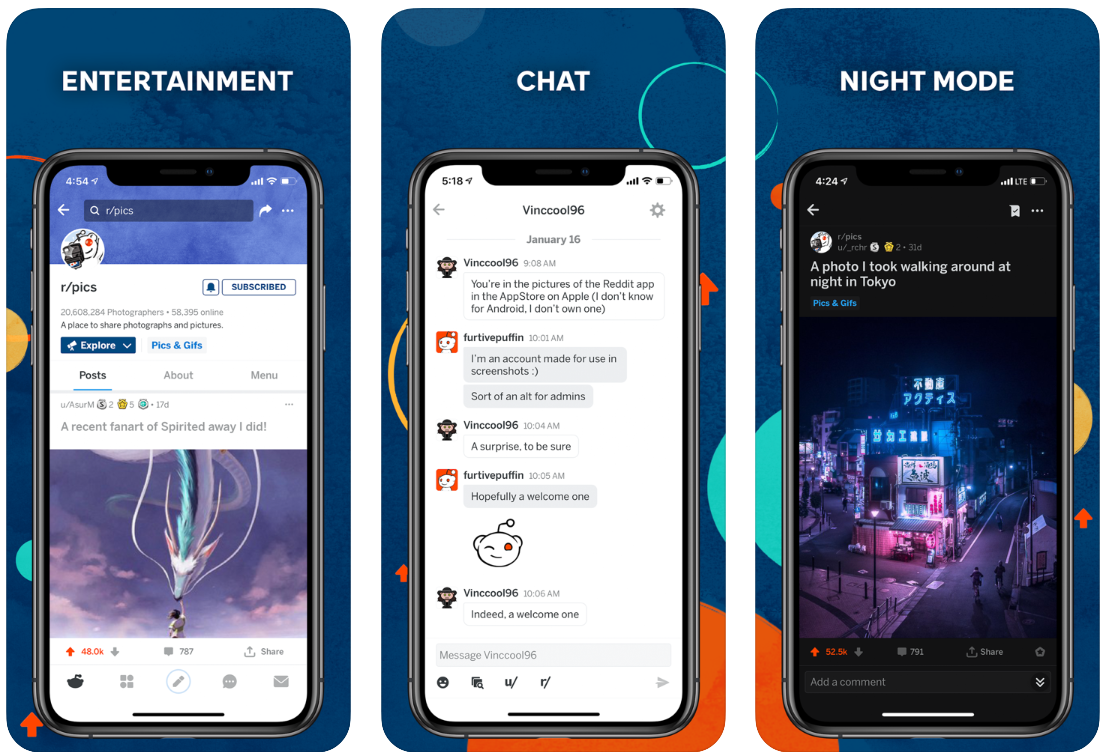
\includegraphics[width=\textwidth]{figures/reddit/reddit_ios.png}
        \caption{Official iOS Reddit application}
        \label{a:fig:reddit_ios}
    \end{figure}
    
    \begin{figure}[ht]
        \centering
             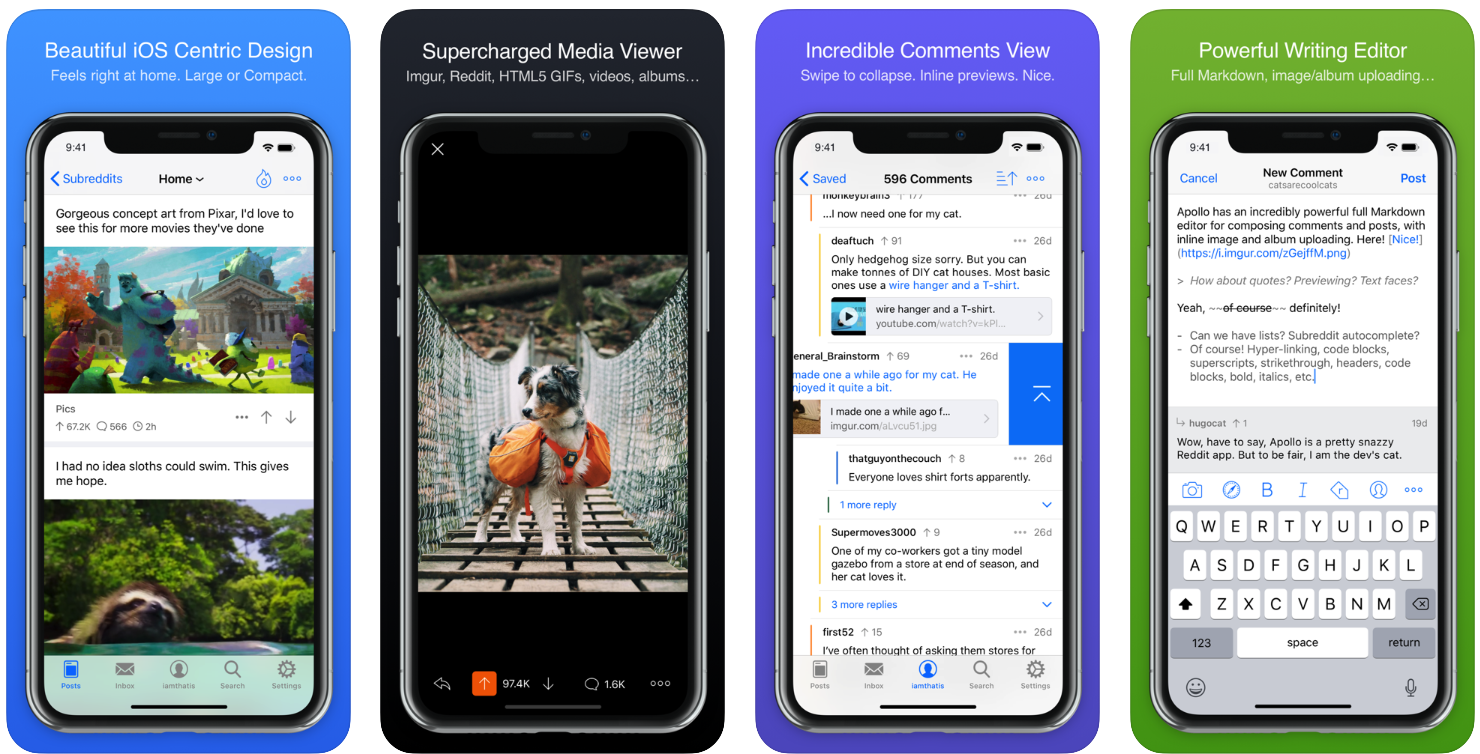
\includegraphics[width=\textwidth]{figures/reddit/reddit_apollo.png}
        \caption{Apollo for Reddit, an unofficial iOS application}
        \label{a:fig:reddit_apollo}
    \end{figure}

\begin{landscape}
\chapter{UML diagrams} \label{a:uml}
    \begin{figure}[ht]
        \centering
             
\includegraphics[width=\linewidth]{figures/uml/system.pdf}
        \caption{A simplified UML diagram of the entire system}
        \label{a:fig:uml}
    \end{figure}
    
    \begin{figure}[ht]
        \centering
             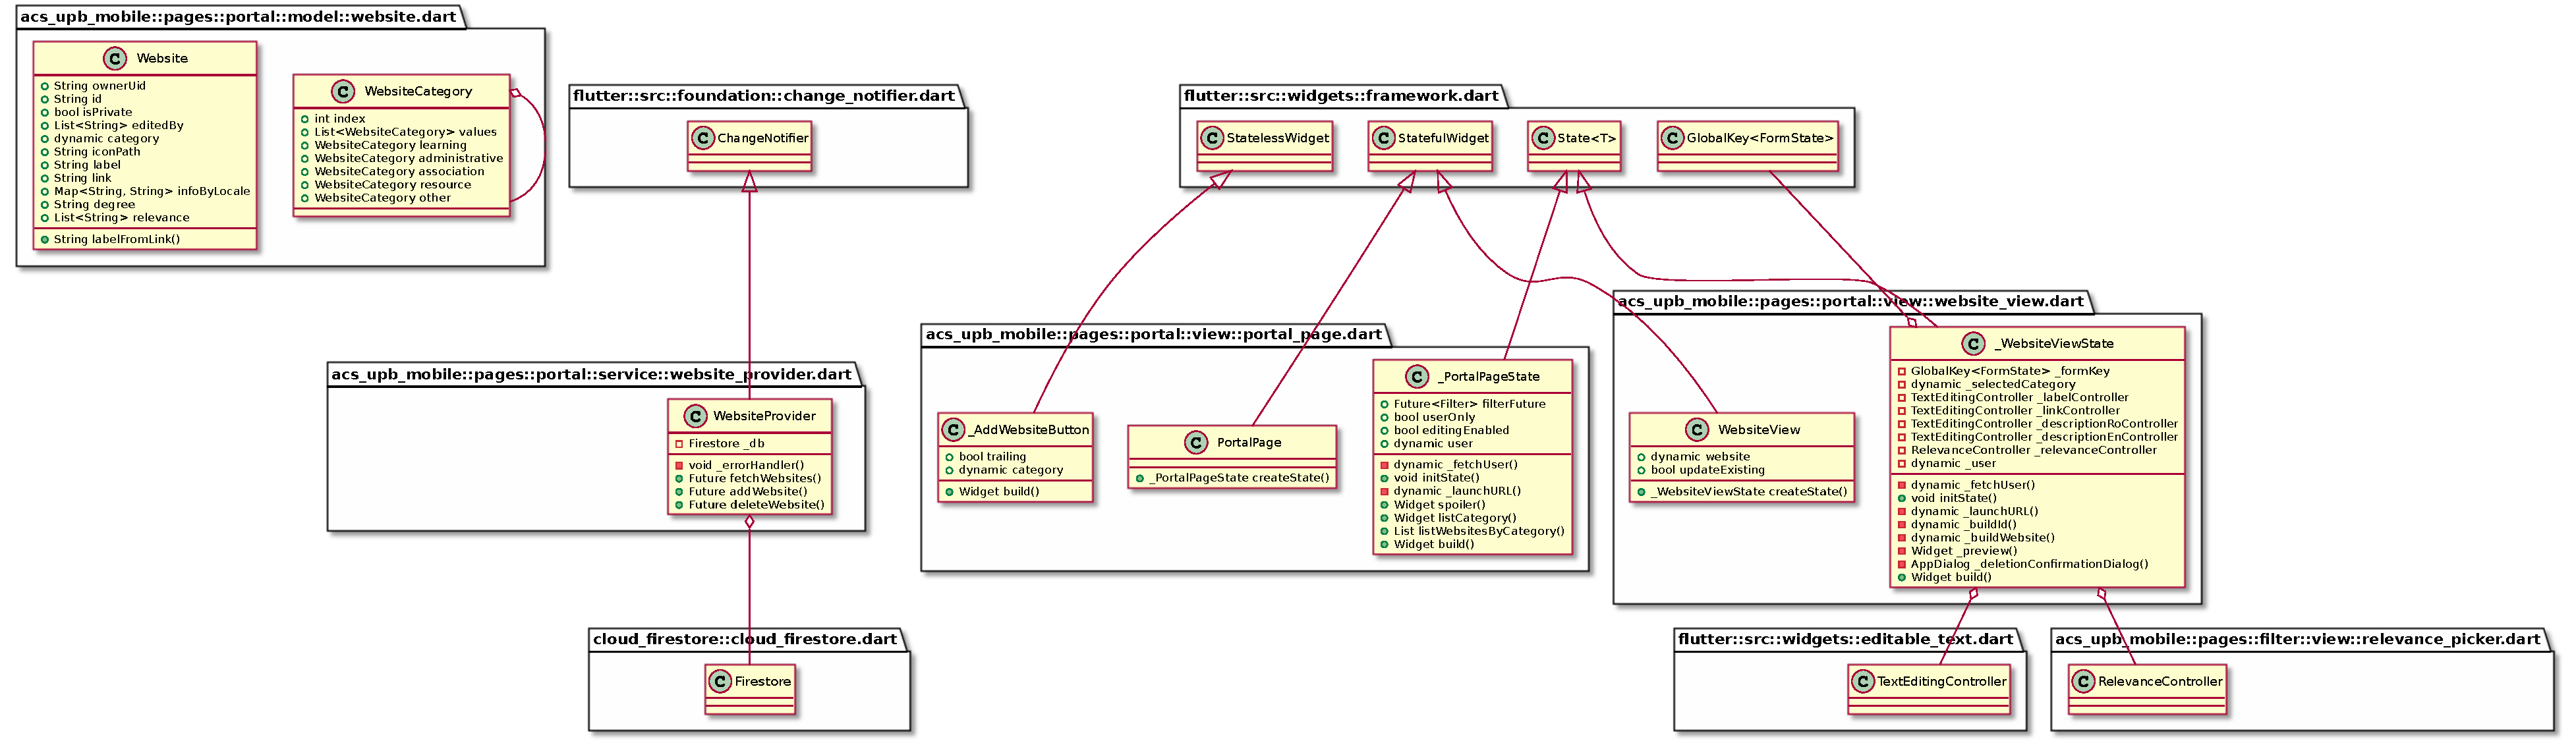
\includegraphics[width=\linewidth]{figures/uml/portal.pdf}
        \caption{Diagram of the portal page}
        \label{a:fig:uml_portal}
    \end{figure}
    
    \begin{figure}[ht]
        \centering
             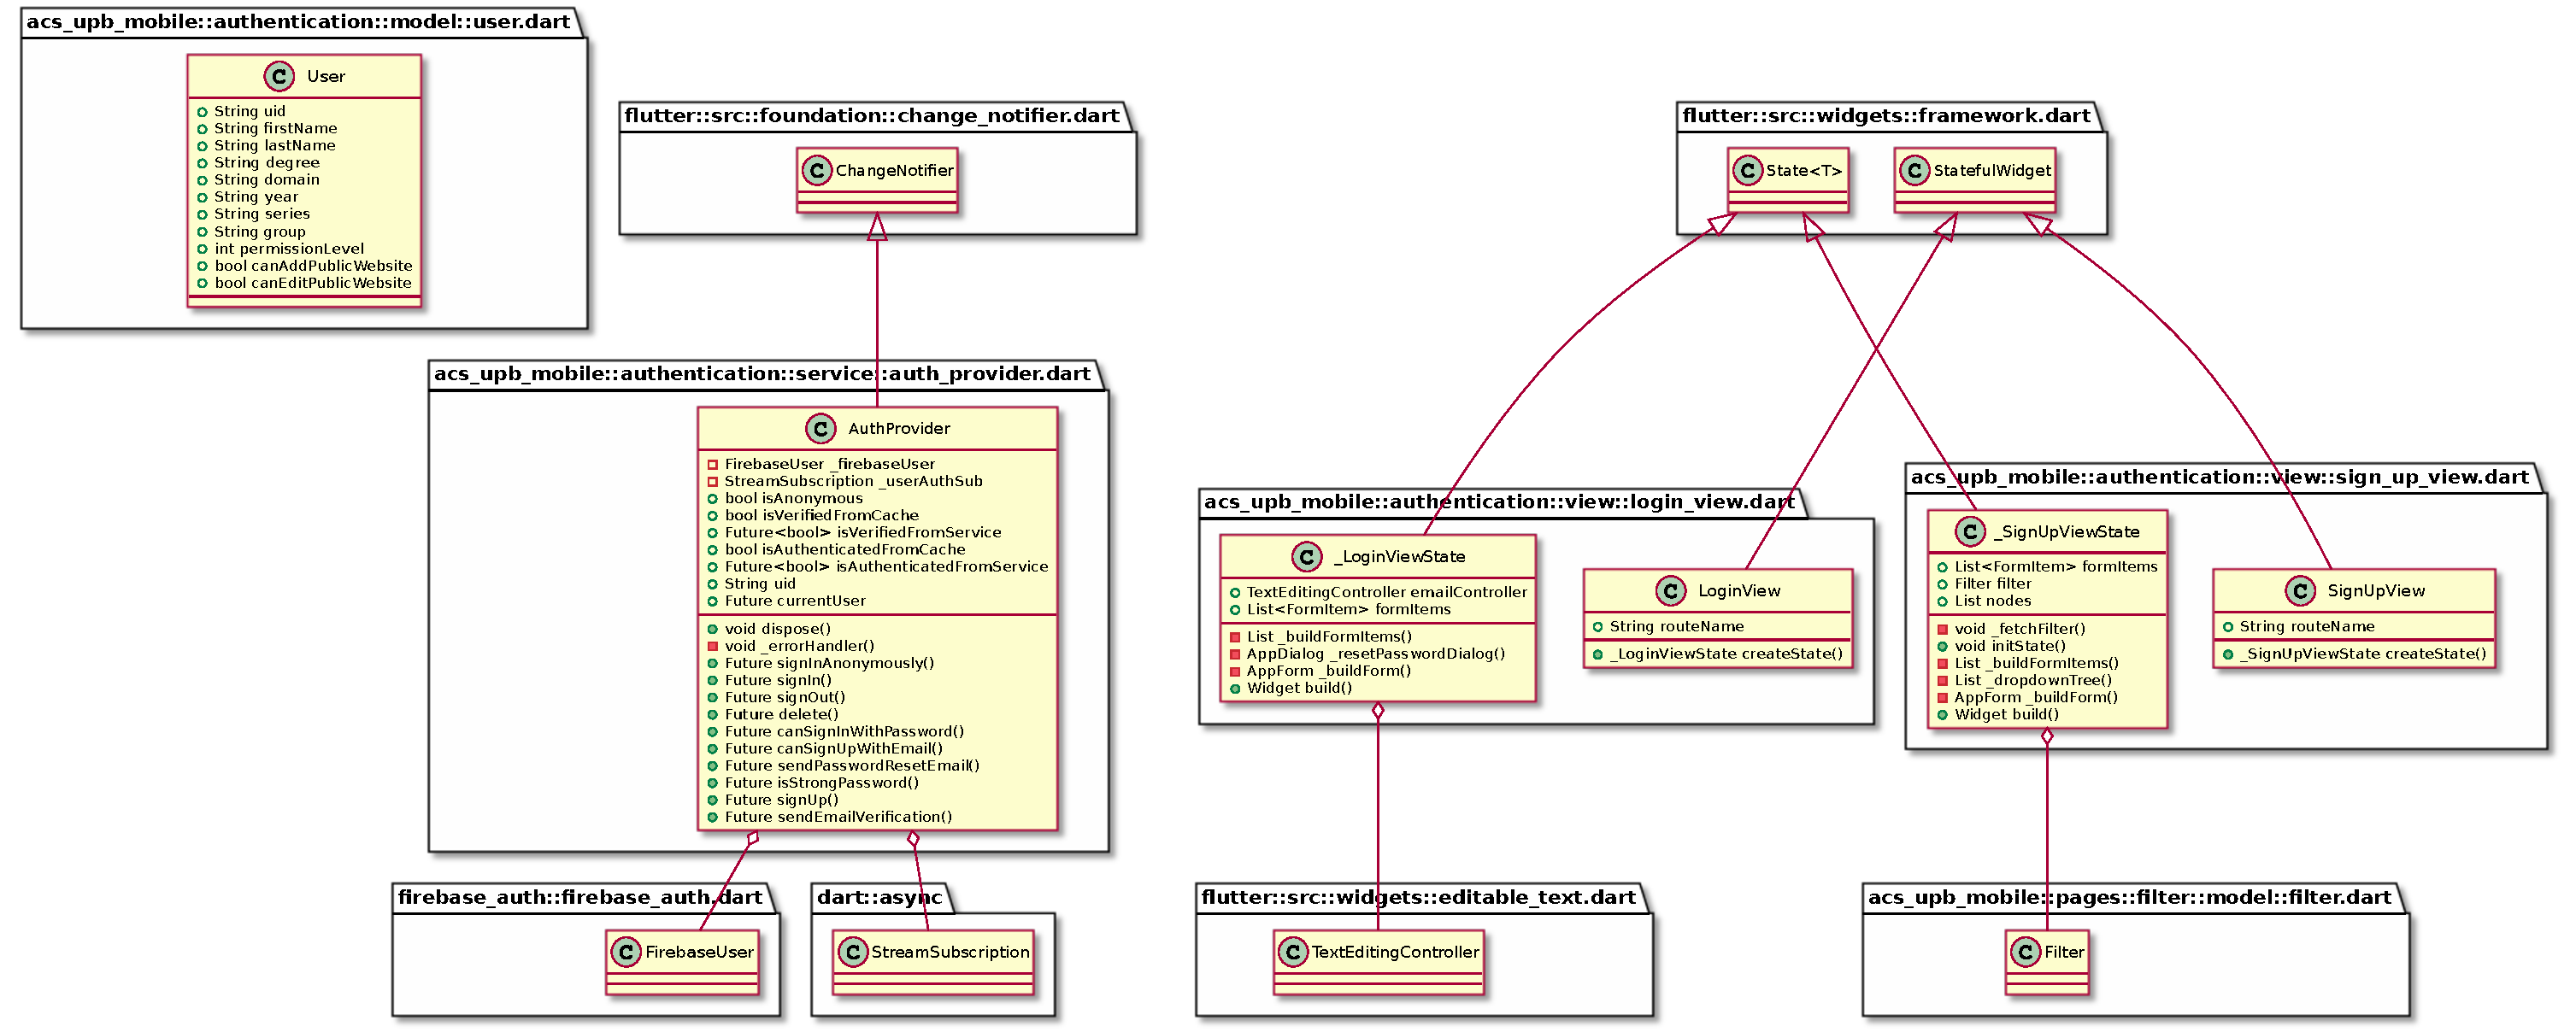
\includegraphics[width=\linewidth]{figures/uml/authentication.pdf}
        \caption{Diagram of the authentication system}
        \label{a:fig:uml_authentication}
    \end{figure}
\end{landscape}
    
\addtocontents{toc}{\endgroup}